\documentclass{scrartcl}
\usepackage[]{geometry}
% \usepackage[parfill]{parskip}
\usepackage[utf8]{inputenc}
\usepackage{graphicx}
    
\usepackage{amsmath,amssymb,amsfonts,amsthm}
\usepackage{chronology}
\usepackage{csvsimple}


\usepackage{hyperref}
\hypersetup{colorlinks,linkcolor=black,citecolor=black,urlcolor=black,linktoc=all,}

\begin{document}
\pagestyle{plain}

\begin{titlepage}
\begin{center}
\vspace*{1cm}
\huge
\textbf{Style-Specific Beat Tracking with\\ Deep Neural Networks}
\vspace{2.0cm}

\Large
\textbf{Julius Richter}
\vspace{0.8cm}

\includegraphics[width=0.3\textwidth]{figures/tu_logo.pdf}

\vspace{0.4cm}
Audio Communication Group\\
Technische Universität Berlin\\
\vspace{2.5cm}
This thesis is submitted for the degree of\\
\emph{Master of Science}

\vspace{2.5cm}
First Supervisor: Prof. Dr. Stefan Weinzierl \\
Second Supervisor: Prof. Dr. Klaus-Robert Müller\\
\vspace{1.5cm}
\today
\end{center}
\end{titlepage}


\tableofcontents
\newpage


\section{Introduction}

\begin{itemize}
\item Rhythm is indispensable for music.
\item Rhythm is music’s central organizing structure. It orders the movement of musical patterns in time. 
\item A fundamental research topic in music information retrieval is the automatic extraction of beat locations from music signals. 
\item The aim of a beat tracker is to recover a sequence of time instants from a musical input that are consistent with the times when a human might tap their foot \cite{Ellis2007}. 
\item Beat tracking is an important initial step in computer emulation of human music understanding, since beats are fundamental to the perception of (Western) music.
\item The goal of beat tracking is to construct a computational algorithm capable of extracting a symbolic representation which correspond to the phenomenal experience of beat or pulse of a human listener.
\item The primary information required for beat tracking is the onset times of musical events, i.e., musical notes and percussive sounds, and this is sufficient for music of low complexity and little variation in tempo.
\item The interpretation of beat is one of the most fundamental aspects of musical intelligence.
\item A naive approach to describe the rhythm of musical data is to specify an exhaustive and accurate list of onset times, maybe together with some other musical features characterizing those event, e.g., durations, pitches and intensities. However, such a representations lacks abstraction. Diverse media used for rhythm transmission suffer a trade-off between the level of abstraction and the comprehensiveness of the representation. Standard (Western) music notation provides an accepted method for communication a composition to a performer, but it has little value in representing the interpretation of a work as played in a concert. On the other hand, an acoustic signal implicitly contains all rhythmic aspects but provides no abstraction whatsoever \cite{Gouyon2005}.
\item The main goal in automatic rhythm description is the parsing of acoustic events that occur in time into the more abstract notions of metrical structure, tempo and timing. A major difficulty is the inherent ambiguity of rhythm.
\item How well does the proposed model generalize to different musical styles?
\item The pattern recognition task is a nontrivial problem due to the wide variability of rhythm in music. 
\item Beat tracking can be tackled using handcrafted rules or heuristics for distinguishing on which time instant a beat is based on the properties of the audio signal. In practice such an approach leads to a proliferation of rules and of exceptions to the rules and so on, and invariably gives poor results. Far better results can be obtained by adopting a machine learning approach in which a large set of $N$ tracks $\{\mathbf x^{(1)}, \dots, \mathbf x^{(N)}\}$ called a training set is used to tune the parameters of an adaptive model. The beat instants of the tracks are known in advance, typically by inspecting them individually and hand-labeling them. So for every track $\mathbf x$ there is a target vector $\mathbf y$. The result of the machine learning algorithm can be expressed as a function $\hat{\mathbf y} = \phi (\mathbf x)$ which takes a new track $\mathbf x$ as input and that generates an output vector $\hat{\mathbf y}$, encoded in the same way as the target vectors. The precise form of the function $\phi (\mathbf x)$ is determined during the training phase, on the basis of the training data. Once the model is trained it can then determine the identity of new tracks, which are said to comprise a test set. The ability to categorize correctly new examples that differ from those used for training is known as generalization. In practical applications, the variability of the input vectors will be such that the training data can comprise only a tiny fraction of all possible input vectors, and so generalization is a central goal in pattern recognition. 
\item Applications in which the training data comprises examples of the input vectors along with their corresponding target vectors are known as supervised learning problems. 
\end{itemize}




\paragraph{Difficulties of Beat Tracking}
\label{sec:difficulties}
\begin{itemize}
\item It is difficult to reliably extract high-level rhythm related features from musical excerpt having properties such as soft onsets, heavy syncopation or making use of expressive timing (e.g. rubato playing) \cite{Quinton2016}.
\item The principal reason that beat tracking is intrinsically difficult is that it is the problem of inferring an original beat structure that is not expressed explicitly. The degree of beat tracking difficulty is therefore not determined simply by the number of musical instruments performing a musical piece, it depends on how explicitly the beat structure is expressed in the piece. However, it is very difficult to measure its explicitness because it is influenced from various aspects of the songs.
\item The larger the number of syncopation, the greater the difficulty of beat tracking (quantitative measure: power-difference measure \cite{Goto1999}).
\item The main reason that different tendencies with regard to the explicitness with which the beat structure is indicated.
\item There is not necessarily a specific sound that directly indicates the position of beats. In fact, a musical beat may not directly correspond to a real sound, there may even be no signal on a beat. 
\item absence of a clear rhythmic structure (Classical music)
\item soft onsets
\item blurred note transitions (e.g. classical music dominated by string instruments)
\item heavy syncopation
\item expressive timing (e.g. rubato playing)
\item the problem of 'octave errors' (detecting double or half time the rate of the ground truth)
\item Acoustic signals consist of sound of various kinds of instruments.
\item The onsets of notes are difficult to obtain, unlike the case of MIDI signals, where there is no such problem.
\item A beat may not directly correspond to a real sound. It is a perceptual concept that human feels in music. 
\item Multiple interpretations of beats are possible at any given time.
\item There is no simple relationship between polyphonic complexity -- the number and timbres of notes played at a single time -- in apiece of music, and its rhythmic complexity or pulse complexity \cite{Scheirer1998}. There are pieces and styles of music which are texturally and timbrally complex, but have straightforward, perceptual simple rhythms; and there also exist music which deal in less complex textures but are more difficult to rhythmically understand an describe.
\item The complexity of grouping harmonic partials together to form notes, and determining the onset times of those.
\item For this reason Cemgil et al. \cite{Cemgil2001} define music transcription as the extraction of an \emph{acceptable} music notation.
\item There is no canonical form for representing rhythm, and lacking this ground truth, it is difficult, if not impossible, to provide a meaningful quantitative comparison of the various computer systems. Therefore we need a common database of test music labeled with the ground truth on which the systems are tested. 
\end{itemize}



% Quantify the difficulty of beat tracking with indicators such as
% \begin{itemize}
% \item beat strength [Tzanetakis2002]
% \item pulse clarity [Lartillot2008]
% \item entropy of a cyclic tempogram [Grosche2010] as an indicator of the tempo salience  
% \end{itemize}


\paragraph{Applications of Beat Tracking}
\begin{itemize}
\item Estimating the beats of an musical audio opens new possibilities for a wide range of applications. 
\item Beat tracking can be used to automate time-consuming tasks that must be completed in order to synchronize events with music. 
\item Video and audio editing, e.g., the visual track can be automatically synchronized with an audio track using beat tracking.
\item Stage light control. In live performances, beat tracking is useful in the control of stage lighting by a computer. For instance, various properties of lighting such as color, brightness, direction, and effect can be changed in time to the music.
\item Visualization, e.g., time-grid representation in audio sequencers.
\item Musical interaction systems \cite{Robertson2007}
\item Content-based audio effects, for multimedia or interactive performances or studio post-production
\item Beat-driven real-time computer graphics.
\item Temporal segmentation to higher level MIR tasks such as chord estimation for harmonic description \cite{Bello2005b}.
\item Long-term structural segmentation of audio \cite{Bartsch2005}
\item performance analysis investigates the interpretation of musical works, e.g., the performer's choice of tempo and expressive timing. 
\item In audio content analysis, beat tracking is important for automatic indexing and content-based retrieval of audio data, such as in multimedia databases and libraries.
\item Automatic transcription and score extraction from performance data 
\item Music similarity
\item Time-stretching of audio loops
\item Beat tracking can provide computers the ability to participate intelligently in live performances in real time and join the ensemble.
\item synchronization of a musical performance with computers or other devices
\item Commercial devices already exist that attempt to extract a MIDI clock from an audio signal, indication both the tempo and the actual location of the beat. Such MIDI clocks can the be used to synchronize other devices such as drum machines or audio effects, enabling a new range of beat-synchronized audio processing.
\item Automatic playlist generation, where a computer is given the task to choose a series of audio tracks from a track database in a way similar to what a human deejay would do. The track tempo is a very important selection criterion in this context, as deejays will tend to string tracks with similar tempi back to back. Furthermore, deejays also tend to perform beat-synchronous cross-fading between successive track manually, slowing down or speeding up one of the tracks so that the beat in the two tracks line up exactly during the cross-fade. This can easily be done automatically once the beats are located in the two tracks.
\end{itemize}



\newpage
% Rename to 'History of Beat Tracking'?
\section{Related Work}

This chapter is an overview of related work that fostered the development of beat tracking in musical audio. The task of automatic rhythm detection has been well established over the last thirty-five years and beat tracking algorithms have constantly improved in performance. A chronology with the most influential work is shown in Fig. \ref{fig:history}.

\begin{figure}[htpb]
\centering
\begin{chronology}[5]{1984}{2024}{\textwidth}[\textwidth]
\event{1985}{Schloss \cite{Schloss1985}}
\event{1990}{Allen and Dannenberg \cite{Allen1990}}
\event{1994}{Goto and Muraoka \cite{Goto1994}}
\event{1998}{Scheirer \cite{Scheirer1998}}
\event{2001}{Cemgil et al. \cite{Cemgil2001}, Dixon \cite{Dixon2001}}
\event{2003}{Laroche \cite{Laroche2003}}
\event{2005}{Klapuri et al. \cite{Klapuri2005}}
\event{2007}{Davies and Plumbley \cite{Davies2007}}
\event{2009}{Peeters \cite{Peeters2009}}
\event{2011}{Böck and Schedl \cite{Boeck2011}}
\event{2014}{Böck et al. \cite{Boeck2014}}
\eventmarker{2015}{Krebs et al. \cite{Krebs2015}}
\eventlabel{2016}{Krebs et al. \cite{Krebs2015}}
\event{2019}{Davies and Böck \cite{Davies2019}}
\end{chronology}
\caption{Time-line with the history of beat tracking.}
\label{fig:history}
\end{figure}

The traditional approach of beat tracking consists of extracting features from an audio signal to obtain a feature list. These features range from note onsets, as time, duration and pitch, to frequency-based signal features and they convey predominant information relevant to rhythmic analysis. The feature extraction is usually followed by a periodicity detection stage and the estimated periodicities subsequently determine the beat times using a temporal decoding strategy. Nevertheless, the recent trend in beat tracking is a shift away from purely signal processing approaches towards data-driven approaches incorporating machine learning. In the following, most influential approaches are represented chronologically. 

% \begin{itemize}
% \item 
% \item The recent trend in music information retrieval to shift away from purely signal processing approaches to those incorporating machine learning. 
% \item Overview: Signal processing $\rightarrow$ data-driven approaches
% \item traditional approach of precessing a list of onsets
% \item new approach use artificial neural networks to perform a frame by frame beat classification.
% \item The first analysis step is the creation of a feature list, i.e. the parsing, of filtering, of the data at hand into a sequence of features. These features range from note onset features (as time, duration and pitch), to frae-based signal features, and they convey the predominant information relevant to rhythmic analysis.
% \item The extraction of note onsets times for rhythmic analysis is ubiquitous in the litarature. An exhaustive overview of musical onset detection can be found in \cite{Bello2003}.
% \item Some systems do not focus on note onsents and their features, but refer to a data granularly of a lower lever of abstraction, namely frames. A frame is a short chunk, typically $10\,\text{ms}$ of audio, from which both time and frequency domain features can be computed. Consecutive frames are usually considered with some overlap for smoother analyses, and the analysis step, the hop size, equals the frame size minus the overlap. 
% \end{itemize}


% Should I add Chowning et al. 1984?

Schloss \cite{Schloss1985} proposed one of the earliest work on automatic extraction of rhythmic content from audio in his percussion transcription system. Onsets are detected as peaks in the slope of the amplitude envelope, where the envelope is defined to be equal to the maximum amplitude in each period of the high-pass filtered signal. The period is defined as the inverse of the lowest frequency expected to be present in the signal. The main limitation of the system is that it requires parameters to be set interactively. 

Allen and Dannenberg \cite{Allen1990} extended the musical concept of beat by including two aspects, namely period and phase. Based on that concept, they built a method that uses real-time beam search to allow the beat tracker to consider several possible stages at once. They use a credibility measure so that at any given time there is a set of active states that represent the most credible interpretations for the performance encountered so far. However, the system's reliance on MIDI limited the input source to electronic instruments, and moreover limited its application.

Goto and Muraoka \cite{Goto1994} introduce the first worth mentioning beat tracking system which could process music played on ensembles of a variety of instruments. However, they restricted their system to rock and pop music in which drums maintain the beats. The system leverages the fact that for a large class of popular music, a bass drum and a snare drum usually occur on the strong and weak beats, respectively. In their algorithm, multiple agents estimate beat times according to different strategies in order to examine multiple hypothesis in parallel. All hypotheses are gathered and the most reliable one is selected as the output. This enables the system to follow beats without losing track of them, even if some hypothesis become wrong. Assumptions were made; tempo between 65 and 185 BPM, time-signature is 4/4, tempo stays almost constant. In following developments, Goto \cite{Goto2001} presents a beat tracking system for both music with and without drum-sounds. It uses frequency-domain analysis to detect chord changes, which are assumed to occur in metrically strong positions. This is the fist system to demonstrate the use of high level information in directing the lower-level beat tracking process. The high level information is specific to the musical style, which is a major limitation of the system.  

Scheirer \cite{Scheirer1998} concludes from psychoacoustic studies on beat perception, that amplitude envelopes from a small number of broad frequency channels are sufficient information to rhythmically analyze musical content. He infers that a rhythmic processing algorithm should treat frequency bands separately, combining results at the end, rather than attempting to perform beat tracking on the sum of filter-bank outputs. This leads him to the use of a small number of bandpass filters and banks of parallel comb filters, which function as tuned resonators, to perform periodicity analysis. In the next processing step, the phase of the musical signal is extracted by examining the internal state of the delays of the comb filters. Finally, the phase and the period is used to estimate the beat times as far into the future as desired. One problem with the system is that in order to track tempo changes, the system must repeatedly change its choice of filter, which implies the filters must be closely spaced to be able to smoothly track tempo variations. However, the system applies no continuity constraint when switching between filters.  

Dixon \cite{Dixon2001} processes a sequence of note onset times either extracted from an audio signal or from a symbolic representation within a multi-agent system. Likely tempo hypotheses are derived from clustering inter-onset intervals (IOI), thus encoding aspects of the metrical hierarchy. The hypothesis are used to form multiple beat agents using a paradigm, where each agent has a state consisting of the period and the phase of the beat. The sequence of beat times with the best score to date is selected by the agent. The observations are only processed if they occur around the predicted beat locations, i.e., within a window whose width depends on the pulse period. The algorithm is designed to track beats in expressively performed music.
% add Dixon 2003

% In this framework, 

% \begin{itemize}
% % \item Dixon \cite{Dixon2001} uses histograms of time intervals between similar events. He uses IOI histograms where the bins are not fixed.
% % \item Clusters of similar IOIs are given scores based on the number of elements in the cluster and the amplitudes of ther onsets.
% % \item An ajustment of the scores and cluster representative interval the favours rationally-related cluster
% % \item The computation of the period entails the loss of time localisation, and the phase has to be computed subsequently  during pulse trackking. 
% % \item Uses a fixed tolerance interval of $25\,\text{ms}$ für IOIs
% % \item Presents another multiple hypotheses search, using an agent paradigm, where each agent has a state, consiting of the period and the phase of the pulse, and a history, the sequence of beat times selected to date by the agent. The observations are only processed if they occur around the predicted beat locations, i.e., within a window whose width depends on the pulse period.
% \item Dixon et al. \cite{Dixon2003} employ tolerance intervals proportional to the IOIs, so longer IOIs allow for greater variations.
% \end{itemize} 

Cemgil et al. \cite{Cemgil2001} formulate beat tracking in a probabilistic Bayesian framework where tempo and beat is modeled as a stochastic dynamical system. The system is defined with two hidden state variables, the period and the phase of beat. To this deterministic model, they add a Gaussian random vector whose covariance matrix models the likely tempo variations. State transitions are defined by a simple set of equations that describe how state variables evolve with time. 
Because all noises are assumed to be Gaussian and all relationships between variables are linear, the covariance matrix can be efficiently estimated by a Kalman filter. They also develop the tempogram representation which includes a probability distribution over the period and phase given a list of onset. This probability distribution is proportional to the likelihood of the observed onsets under given period and phase hypotheses, weighted by prior distribution, which is equally distributed, as they consider all tempi to be initially equiprobable. For given periods and phases, the likelihood is computed as the integral over all onsets of the product of a constant pulse track and a continuous representation of the onsets. This implements the assuption that a good pulse track is one which matches all onsets well. The tempogram's marginal probability distribution provides a 1-D representation of periodicities resembling those aforementioned. 
%  will be estimated through a training phase.

% Temperley and Sleater \cite{Temperley1999} use dynamic programming to search the solution space of possible mappings of events to a metrical grid, where the search is guided by a set of preference rules based of GTTM.

Laroche \cite{Laroche2003} initially finds salient features like note onsets, note changes, and percussion hists by calculating the Fourier transform of an audio signal. A nonlinear monotonic compression function is applied to the amplitude spectrum, so high-frequency component is not masked by higher amplitude low-frequency components. To locate fast variations in the frequency domain content, a first-order difference is calculated. All bins are summed together, and the result is half-wave rectified to obtain a positive energy flux signal. A least-squares approach is used to determine the best candidates for the tempo and beat locations. The final step consist of going through the successive tempo analysis frames and finding in each frame the best candidates. To that effect a dynamic programming technique is used. This entails continuity and non-syncopation constraints. 

Klapuri et al. \cite{Klapuri2005} expand upon Scheirer's amplitude envelope and comb filter model. They adopt a more robust registral accent signal across four parallel analysis bands as the input to their system and use comb filter-banks within a probabilistic framework to simultaneously track three metrical levels. These correspond to the tatum, tactus and measure. Analysis can be performed causally an non-causally, and is not restricted to any particular genre, tempo or time-signature. The robustness of the analysis model is due to the probabilistic modeling of the temporal evolution and interaction between each og the three metrical levels analyzed. In a study of audio tempo induction algorithms \cite{Gouyon2006b}, this approach was shown to be most accurate.

Davies and Plumbley \cite{Davies2007} adopt a simpler and more efficient, heuristic approach than the system of Klapuri by embedding context-dependent information directly into the beat period and alignment estimation processes. They use two state model; the first state performs tempo induction and tracks tempo changes, while the second maintains contextual continuity within a single tempo hypotheses. The first state, also called general state, operates in a memoryless fashion, extracting the beat period and beat alignment through a process of repeated induction. In this manner, the two-state model can explicitly model tempo discontinuities while smoothing out odd beat errors during each consistent beat period hypothesis. 

Peeters \cite{Peeters2009} approach is based on a probabilistic framework, in which the beat tracking problem is formulated in a hidden Markov model, that can be efficiently solved with the Viterbi algorithm \cite{Viterbi1967}. An onset-energy-function, time-variable tempo, and meter serves as an input to the system. Beat times are decoded over beat-numbers according to observation and transition probabilities. A beat-template is used to derive the observation probabilities from the signal. For this purpose, a linear discriminant analysis finds the most discriminative beat-template. 
% A significant change was introduced by Eyben who transit from signal processing to data-driven method which utilise the power of machine learning. 

Böck and Schedl \cite{Boeck2011} present the first beat tracking system which is based on artificial neural networks. The network transforms the signal directly into a beat activation function, which represents the probability of a beat at each frame.  As network architecture they use a bidirectional recurrent neural network (RNN) with long short term memory (LSMT) units. The approach is inspired by the good results for musical onset detection \cite{Eyben2010} and extended to suit the needs for audio beat tracking by modifying the input representation and adding a peak detection stage. As input to the network, three filtered magnitude spectra with different window lengths and their first order differences are used. In a peak detection stage, first the periodicity within the activation function is detected with the autocorrelation function to determine the most dominant tempo. The beats are then aligned according to the previously computed beat interval. In this way, erroneously detected beats are eliminated or missing beats are complemented.

Böck et al. \cite{Boeck2014} extend the previous beat tracking system of Böck and Schedl with a multi-model approach to represent different music styles. For this purpose, they use multiple recurrent neural networks, which are trained on certain heterogeneous music styles. The system chooses the model with the most appropriate beat activation function for the input signal and jointly models tempo and phase of the beats with a dynamic Bayesian network. Compared to a reference model, which was trained on the whole training set, the specialized models produce better predictions on input data which is similar to that used for training, but worse predictions on signals dissimilar to the training data.

Krebs et al. \cite{Krebs2015} propose a modified state-space discretization and tempo transition model for the temporal decoding stage with dynamic Bayesian networks. The modification increases beat tracking accuracy and also reduces time and memory complexity. To be consistent with human tempo sensitivity, they propose to make the number of discrete bar positions dependent on the tempo and distribute the tempo states logarithmically across the range of beat intervals. 
% See Section \ref{sec:temporal_decoding} for details.

Davies and Böck \cite{Davies2019} suggest to use a convolutional neural network in form of a temporal convolutional network (TCN) \cite{Bai2018}. In comparison to the recurrent model of Böck et al. \cite{Boeck2014}, the TCN can be trained more efficiently on very large datasets due to parallelization. It requires a smaller number of trainable parameters while achieving state-of-the-art performance. 



\newpage
% basic principles of how humans understand rhythms
% Old: Basic Principles of Rhythm
\section{Rhythm}
\label{sec:perception}

Rhythmic organization is an inherent part of all human activity. As the time structure of music, rhythm is composed of distinct temporal components such as pattern, meter, and tempo. In this chapter, basic principles and definitions of those components of music are explained.  


\subsection{Terminology}

\paragraph{Rhythm} 
In music and music theory, there are many different definitions of rhythm. Generally, rhythm means a movement marked by the regulated succession of strong and weak elements, or of opposite or different conditions \cite{Dictionary1971}. It is regarded as the way in which accented and non-accented notes are grouped in a time unit \cite{Cooper1966}. The definition of Lester \cite{Lester1986} considers the patterns of duration between musical events and has the advantage that events pertaining to various musical qualities, giving rise to the idea that more than one rhythm can be defined for a musical piece. Whereas London \cite{London2001} defines rhythm as the sequential pattern of durations relatively independent of meter or phrase structure. In general, the experience of rhythm involves movement, regularity, grouping, and yet accentutation and differentiation \cite{Handel1989}.


\paragraph{Onset} 
An onset refers to the beginning of a musical note or other sound. Any rhythmic event is basically characterised by an onset time and a salience. They represent the most basic unit of rhythmic information, from which all beat and tempo information is derived. The concept of onsets is related to the concept of transients, but differs in the way that all musical notes have an onset, but do not necessarily include an initial transient. The more salient events are, the more likely to correnspond to beat times than the less salient ones. This tendency for events with greater perceptual salience to occur in stronger metrical positions has been noted by various authors \cite{Lerdahl1985,Povel1985,Parncutt1994}. Lerdahl and Jackenhoff \cite{Lerdahl1985} classify musical accents into three types: phenomenal accents, which come from physical attributes of the signal such as amplitude and frequency; structural accents, which arise from perceived points of arrival and departure such as cadences; and metrical accents, points in time which are perceived as accented due to their metrical position.


\paragraph{Beat} 
The term beat, or more technically the \emph{tactus}, refers to the perceived pulses which are approximately equally spaced and define the rate at which notes in a piece of music are played \cite{Handel1989}. Intuitively, it is often defined as the rhythm listeners would tap their foot to when listening to a piece of music, or the numbers a musician counts while performing. Therefore, the beat is most often designated as a crotchet or quarter note in western notation. In beat tracking, the period of a beat is the time duration between two successive beats, i.e. the reciprocal of the tempo. Whereas the phase determines where a beat occurs with respect to performance time.
% For a specific performance, the beat is defined by the occurance times, beat times, of these pulses.
% The beat of a piece of music is the sequence of equally spaced phenomenal impulses which define a tempo for the music. 


\paragraph{Tempo}
Given a metrical structure, tempo is defined as the rate of beats at a given metrical level. Thus, it corresponds to the frequency of the primary pulse in a rhythmic musical signal. The tempo is commonly expressed as a number of beats per minute (BPM). In order to represent changing tempi, various approaches can be used. If tempo is considered as an instantaneous value, it can be calculated as the inter-beat interval (IOI) measured between each pair of successive beats. A more perceptual plausible approach is to take an average tempo measured over a longer period of time. A measure of central tendency of tempo over a complete musical excerpt is called the basic tempo, which is the implied tempo around which the expressive tempo varies \cite{Repp1994}. The value of tempo as a function of time is called a tempo curve, and can be visualized in a tempogram \cite{Cemgil2001}.


\paragraph{Meter} 
% Metrical level see Dixon 2001

The term meter refers to the regularly recurring patterns and accents such as beats and bars and provides an underlying time frame. Unlike rhythm, meter is a perceptual concept which is inducted from the phenomenally accented points of musical surface \cite{London2004}. The metrical structure is hierarchical, i.e., it involves a ratio relationship between at least two time levels, namely the referent time level, the beat, and a higher order period based on a fixed number of beat periods, the measure \cite{Yeston1976}. Meter is regular and stable, and serves as a kind of enhanced temporal grid, which helps to shape expectations about the future and thus be able to anticipate and predict events in time \cite{Huron2006}. In order to establish a meter, some regularity has to be manifesed in the acoustic signal in the first place. Once meter has established, all other events are perceived with refernce to this regular pattern.  In Lerdahl and Jackendoff's \emph{A Generative Theory of Tonal Music} (GTTM) \cite{Lerdahl1985}, the rhythmic structure in the tonal music of the Western tradtition consits of two independent elements, grouping and meter. Grouping is the manner in which music is segmented at a whole variety of levels from groups of a few notes up to large-scale from of a piece of music. Whereas meter is described as the regular alteration of strong and waek elements in music. The metrical structure deals with durationless points in time, e.g. the beats, which obey some well-defined rules. In the GTTM, meter perception is described as the progress of finding periodicities in the phenomenal and structural accents in a piece of music. It also propose a set of metrical preference rules, based on musical intuitions, which are assumed to guide the listener to plausible interpretations of rhythms. Nonetheless, a major weakness of the GTTM is that it does not deal with the departures from strict metrical timing which are apparent in almost all styles of music. Thus, it is only suitable for representing the timing structures of musical scores, or as an abstract representation of a performance, where expressive timing is not represented.

% Tatum, tactus, measure

% They formalise the distinction objective stucture and the performers conceptualisation of music by defining rules for a ``musical grammar'' which deals separately with grouping structure and metrical structure. While the grouping structure deals with time spans, 

% Beats must be equally spaced. A division according to a specific duration corresponds to a metrical level. There must be a beat of the the metrical structure for every note in a musical sequence. A beat at a high level must also be a beat at each lower level. At any metrical level, a beat which is also abeat at the next higher level is called a downbeat, and other beats are called upbeats. Beats obey a discrete time grid, with time intervals all being multiples of a common duration the smalles metrical level. 

% The rules prefer structures where: beats coincide with note onsets; string beats coincide with onsets of long notes; parallel groups receive parallel metrical structure; and the strogest beat occurs early in the group

% Western music notation provides an objective regular temporal structure underlying musical event occurances and organising them into a hierachical metrical structure \cite{Gouyon2005}. 

% Although meter is visualized as a train of pulses with differnet salience, or durationless events in time which conform to a highly regular pattern of hierarchical accentuation, the onsets of actual musical events does not have to coincide with the ponts in time where those pulses are situated. 

% As contrasted with rhythm in general, beat and and pulse correspond inly to the sense of equally spaced temporal units \cite{Handel1989}. Where meter and rhythm associate with qualities of grouping, hierarchy and a strong/weak dichitimy, pulses in apiece of music are only periodic at a simple level.


% old: Psychoacoustics and Human Perception
\subsection{Rhythm Perception}

The perception of music requires the ability to build a temporally ordered architecture of sound sequences in rapid succession. The complex processes underlying this ability have attracted accelerating research in ethology, developmental cognitive sciences, experimental psychology, musicology, and behavioural neurology.

The perception of beat is a prerequisite to rhythm perception, which in turn is a fundamental part of music perception. More psychologically or cognitively motivated definitions associate rhythm to the perceived patterns generated by recurring events and how they interact and categorized by listeners. Nevertheless, there is no ground truth for rhythm to be found in simple measurement of an acoustic signal. The only ground truth is what human listeners agree to be the rhythmic aspects of the musical content of the signal.

Studies of Povel and Essnes \cite{Povel1985} have demonstrated that beat perception may be explained with a model in which a perceptual clock is aligned with the accent structure of the input. The model relies heavily on structural qualities of the input, such as a sophisticated model of temporal accent, to function. They propose a model of perception of temporal patterns, based on the idea that a listener tries to induce an internal clock which matches the distribution of accents in the stimulus and allows the pattern to be expressed in the simplest possible terms. They use patterns of identical tone bursts at precise multiples of $200\, \text{ms}$ apart to test their theory. 

Jones et al. \cite{Jones1989} propose that perceived rhythm is the result of different attending modes, future-oriented and analytic attending. Future-oriented attending involves anticipatory behaviors to coherent temporal events and their durational patterns. They list the following types of phenomenal accent, which they consider incomplete: note onsets, sforzando, sudden dynamic or timbral changes, long notes, melodic leaps and harmonic changes. However, they give no indication as to how these factors might be compared or combined, either quantitatively (absolute values) or qualitatively (relative strengths). Each pair of events in a rhythmic sequence initially contributes to the salience of a single pulse sensation, an emphasis occurs, and later that pulse sensations can enhance the salience of other consonant pulse sensations \cite{Parncutt1994}. One may understand the ``initially'' above as an indication not to implement influential schemes between metrical levels in the induction process, but imdeed to do it in the tracking process. This is also in agreement with the Dynamic Attending Theory \cite{Jones1989}, which proposes that humans spontaneously focus on a reference level of periodicity, and they can later switch to other levels to track events occurring at different time spans, e.g., longer span harmony changes, or a particular shorter-span fast motive. Drake and Bertrand \cite{Drake2001} advocate a universal predisposition toward simple duration ratio, and claim that humans tend to hear a time interval as twice as long or short as previous intervals. 

From psychoacoustic demonstration on beat perception it can be shown that certain kinds of signal manipulations and simplifications can be performed without affecting the perceived pulse content of a musical signal. An amplitude-modulated noise constructed by vocoding a white noise signal with the sub-band envelopes of a musical signal is sufficient to extract pulse and meter. The simplified signal is created by performing a frequency analysis of the original signal by processing it through a filter-bank of bandpass filters, or grouping FFT bins together. Thus it seems that separating the signal into sub-bands and maintaining the sub-band envelopes separately is necessary to do accurate rhythmic processing. This fact leads to the hypotheses that some sort of cross-band rhythmic integration, not simply summation across frequency bands, is performed by the auditory system to perceive rhythm \cite{Scheirer1998}.


The perception of tempo exhibits a degree of variability. It is not always correct to assume that the denominator of the time signature corresponds to the ``foot-tapping'' rate, nor to the actual ``physical tempo'' that would be an inherent property of audio flows \cite{Drake1999}. Differences in human perception of tempo depend on age, musical training, musical preferences and general listening context, e.g., tempo of a previously heard sequence, listener's activity, instant of the day \cite{Drake1993,Drake2000,Drake2000b}. Nevertheless, these differences are  far from random. They most often correspond to a focus on a different metrical level, e.g., differences of half or twice the inter-beat interval or one-third or three times the inter-beat interval. Perception research has shown that with up to $40\,\text{ms}$ difference in onset times, two tones are heard as synchronous, and for more than two tnoes, the threshold is up to $70\,\text{ms}$ \cite{Handel1989}. Rhythmic information is provided by IOIs in the range of approcimately $50\,\text{ms}$ to $2\,\text{s}$ \cite{Handel1989}. Experiments on the tempo sensitivity on humans have shown that the ability to notice tempo changes is proportional to the tempo, with the JND (just noticable difference) beeing around 2-5\% \cite{Drake1993}.

Rhythmic response is crucially a phased phenomenon, in contrast to human pitch recognition, which is only sensitive to signal phase under certain unusual conditions. Tapping on the beat is not at all the same as tapping against the beat or slightly ahead of or behind the beat, even if the frequency of tapping is accurate \cite{Scheirer1998}. Although in the brains of performers music is temporally organized according to its hierarchical beat structure, this structure is not explicitly expressed in music; it is implied in the relations among various musical elements which are not fixed and which are dependent on musical genres or pieces. Expressive timing is generated from performers' understanding of the musical structure and general knowledge of music theory and musical style \cite{Clarke1999}. However, there is no precise mathematical model of expressive timing, and the complexity of musical structure from which timing is derived, coupled with the individuality of each performer and performance, makes it impossible to capture musical nuance in the form of rules \cite{Dixon2001}. Nevertheless, expressive reductions in tempo are more common and more extreme than tempo increases \cite{Repp1994}. 


% change transition prob in HMM


% A listener who cannot identify chord names can nevertheless percieve chord changes.

% Many works in musicpsychology attempt to group musical onsets together into a rhythmic context, i.e., to construct a model which subsumes multiple onsets separated in time into a rhythmic clock, hierachy, grouping, or oscillatory model.

\newpage

% Old: Foundations of Machine Learning
\section{Machine Learning}

Machine learning is subset of artificial intelligence (AI) and deals with algorithms and statistical models that computer systems use to perform a specific task without using explicit instructions, relying on patterns and inference instead. It is essentially a form of applied statistics with increase emphasis on the use of computers to estimate complicated functions and a decreased emphasis on providing confidence intervals around these functions \cite{Goodfellow2016}. On the other hand, pattern recognition is concerned with the automatic discovery of regularities in data, and to take actions such as classifying the data into different categories. Both fields, machine learning and pattern recognition are strongly connected with each other, and together they have undergone a substantial development over the past twenty-five years \cite{Bishop2006}.

Most machine learning algorithms can be divided into the categories of \emph{supervised learning} and \emph{unsupervised learning}. Supervised learning algorithms build a mathematical model of a set of data that contains both the inputs and the desired outputs. Supervised learning algorithms include classification and regression. Unsupervised learning algorithms take a set of data that contains only inputs, and find structure in the data, like grouping or clustering of data points. 

Machine learning tasks are usually described in terms of how the machine learning system should process an example $\mathbf x \in \mathbb R^n$, where an example is a collection of $n$ features $x_i$ that have been quantitatively measured from some object or event. Many kinds of tasks can be solved with machine learning, e.g. classification, regression, transcription, machine translation, synthesis, and sampling, just to name a few.

In this thesis, the focus is on supervised sequence modeling and classification. In the following, basic concepts of machine learning are described. 

% Old: Sequence Modeling
\subsection{Sequence Modeling}
In machine learning, the term sequence modeling encompasses all tasks where sequences of data are transcribed with sequences of discrete labels. Supervised sequence modeling refers specifically to those cases where a set of hand-transcribed sequences is provided for algorithm training. What distinguishes such problems from the traditional framework of supervised pattern classification is that the individual data points cannot be assumed to be independent. Instead, both the inputs and the labels form strongly correlated sequences \cite{Graves2012}.

Given an input sequence $\mathbf x_{1:T} = \mathbf x_1, \dots, \mathbf x_T$ with sequence length $T$, a sequence model is any function $f: \mathcal X^T \rightarrow \mathcal Y^T$, such that
\begin{align}
\mathbf y_{1:T} = \mathbf y_1, \dots, \mathbf y_T = f(\mathbf x_1,\dots, \mathbf x_T)
\end{align}
where vector $\mathbf x_t \in \mathbb R^n$ is the input at time step $t$, and $\mathbf y_t \in \mathbb R^m$ should only depend on $\mathbf x_{1:t}$ and not on $\mathbf x_{t+1:T}$, i.e., no leakage of information from the future. This causality constraint is essential for autoregressive modeling. 

% Thus $\mathbf x_{1:T} \in \mathbb R^{T \times n}$.

The goal of learning in the sequence modeling setting is to find a network $f$ that minimizes some expected loss between the actual outputs and the predictions, 
\begin{align}
L \big( \mathbf y_1, \dots, \mathbf y_T, \, f(\mathbf x_1,\dots, \mathbf x_T) \big) \stackrel{\text{!}}{=} \min
\end{align}
where the sequences and outputs are drawn according some distribution $p_{\text{data}}(\mathbf x,\mathbf y)$.

For most deep learning practitioners, sequence modeling is synonymous with recurrent networks. For example, the sequence modeling chapter in a standard reference on deep learning is titled ``Sequence Modeling: Recurrent and Recursive Nets'' \cite{Goodfellow2016} capturing the common association of sequence modeling and recurrent architectures. Recent results indicate that convolutional architectures can outperform recurrent networks. Concluding from an empirical evaluation of generic convolutional and recurrent networks for sequence modeling, Bai et al. \cite{Bai2018} assert, that the common association between sequence modeling and recurrent networks should be reconsidered, and convolutional networks should be regarded as a natural starting point for sequence modeling tasks.

% Sequence modeling include polyphonic music modeling \cite{Oord2016}, word- and character-level language modeling.
% settings such as auto-regressive prediction, where we try to predict some signal given its past, by setting the target output to be simply the input shifted by ome time step


\subsection{Feature Extraction}

For most practical applications, the original input variables are typically preprocessed to transform them into a new space of variables, where it is hoped the pattern recognition problem will be easier to solve. This preprocessing stage is sometimes also called feature extraction. New test data must be preprocessed using the same steps as the training data. Preprocessing might also be performed in order to speed up the computation, for example, if the goal is a real-time application the algorithm should be computationally feasible. Yet, the aim of feature selection is to find features in the input which preserve useful discriminatory information. Usually, the number of features is smaller than the number of input variables, thus a preprocessing is a form of dimensionality reduction. 

% Dimension reduction

% Many artificial intelligence tasks can be solved by designing the right set of features to extraxt for that task, then providing theses features to a simple machine learning algorithm. \cite{Goodfellow2016}


\subsection{Performance Measure}

To evaluate the abilities of a machine learning algorithm, we must design a quantitative measure of its performance. Usually the performance measure is specific to the task being carried out by the system. For the task of classification, the accuracy of the model is often measured. Accuracy is the proportion of examples for which the model produces the correct output. The choice of performance measure may seem straightforward and objective, but it is often difficult to choose a performance measure that corresponds well to the desired behavior of the system. 

\paragraph{Loss Function}
\begin{itemize}
\item Cross entropy is defined for two probability distributions $p$ and $q$ as
\begin{align}
H(p,q) = - \sum_{x \in \mathcal X} p(x) \log q(x).
\end{align} 
\item In machine learning cross entropy can be used as a loss function to measures the performance of a classification model. The probability $p_{i}$ is the true label (binary indicator 0 or 1), where as the distribution $q_{i}$ is the predicted value of the current model. 
\end{itemize}



% Old: Architectures
\subsection{Model Selection}

In practical applications, the values of the model's parameters are determined by learning, and the principle objective in doing so is usually to achieve the best predictive performance on new data. Furthermore, as well as finding the appropriate values for complexity parameters within the model, one wish to consider a range of different types of model in order to find the best one for a particular application. 

The performance on the training set is not a good indicator of predictive performance on unseen data due to the problem of over-fitting. If data is plentiful, then one approach is simply to use some of the available data to train a range of models, or a given model with a range of values for its complexity parameters, and then to compare them on independent data, also called the validation set, and select the one having the best predictive performance. If the model design is iterated many times using a limited dataset, then some over-fitting to the validation data an occur and so it may be necessary to keep aside a third test set on which the performance of the selected model is finally evaluated. 


\begin{itemize}
\item Given a sequence modeling task or dataset, which architecture should one use?
\item Bai et al. \cite{Bai2018} show that a simple convolutional architectures outperforms canonical recurrent networks such as LSTMs across a diverse range of tasks and datasets, while demonstrating longer effective memory. Is it also the case in beat tracking?
\end{itemize}


\subsection{Optimization}

Most machine learning algorithms involve optimization which refers to the task of minimizing an objective function $f(\mathbf x)$ by altering the arguments $\mathbf x$. The goal of optimization is to find an optimal $\mathbf x^*$, such that
\begin{align}
\mathbf x^* = \arg \min f(\mathbf x)
\end{align} 
Given the function $y=f(x)$, where both $x$ and $y$ are real numbers, the derivative $f'(x)$ is useful for minimizing this function because it indicates how to change $x$ in order to make a small improvement in y. Thus, by moving $x$ in small steps with the opposite sign of the derivative, $f(x)$ is reduced. This technique is called gradient decent \cite{Cauchy1847}. When $f'(x)=0$, the derivative provides no more information about which direction to move and the function reaches a stationary point. Stationary points are classified into three kinds. A local minimum is a point where $f(x)$ is lower than at all neighboring points, and higher for a local maximum respectively. The third kind is known as saddle points where the derivative of the function has the same sign on both sides of the stationary point.  

In the context of machine learning, the objective function has many local minima that are not optimal and many saddle points surrounded by very flat regions. All of this makes optimization difficult, especially when the input to the function is multidimensional. Therefore, it is usually sufficient to find  a value of $f$ that is very low but not necessarily minimal in any formal sense. Thus, in gradient decent we decrease $f$ by moving in the direction of the negative gradient to propose a new point
\begin{align}
\mathbf x' = \mathbf x - \mu \,\nabla_{\mathbf x}f(\mathbf x)
\end{align} 
where $\mu$ is the learning rate, a positive scalar determining the size of the step, and $\nabla_{\mathbf x}$ refers to the gradient with respect to the input $\mathbf x$.


\paragraph{Stochastic Gradient Decent}
Stochastic gradient descent (SGD) is an extension of the basic gradient descent algorithm. A recurring problem in machine learning is that large training sets are necessary for good generalization. At the same time, large learning sets are also more computationally expensive. Instead of using the whole learning set, a small set called minibatch is used to estimate the gradient
\begin{align}
\mathbf g = \frac{1}{N} \,\nabla_{\boldsymbol \theta} \sum_{i=1}^M L(\mathbf x^{(i)}, y^{(i)}, \boldsymbol \theta)
\end{align}  
where $L$ is the per-example loss depending on the input $\mathbf x$, the target $y$, and the model parameters $\boldsymbol \theta$. The minibatch size $M$ is typically chosen to be a relatively small number of examples, ranging from one to a few hundred \cite{Goodfellow2016}. Larger batches provide a more accurate estimate of the gradient, but with less than linear return. Multicore architectures are usually underutilized by extremely small batches. This motivates using some absolute minimum batch size, below which there is no reduction in the time to precess a minibatch. Small batches can offer a regularization effect \cite{Wilson2003}, due to the noise they add to the learning process. Generalization error is often best for a batch size 1. Training with such a small batch size might require a small learning rate to maintain stability because of the high variance in the estimate of the gradient. The total runtime can ba very high as a result of the need to make more steps, both because of the reduced learning rate and because it takes more steps to observe the entire training set. 

\paragraph{Back-Propagation}
When a feedforward neural network takes an input $\mathbf x$ and produce an output $\hat{\mathbf y}$, information flows forward through the network, which is called forward propagation. During training, forward propagation can continue onward until it produces a scalar loss $L(\boldsymbol \theta)$. The back-propagation algorithm \cite{Rumelhart1988} allows the information from the loss to then flow backward through the network in order to compute the gradient. Computing an analytical expression for the gradient is straightforward, but numerically evaluationg such an expression can be computationally expensive. The back-propagation algorithm does so using a simpe and inexpensive procedure. To obtain an algebraic expression for the gradient of a scalar it recursively applies the chain rule with respect to any node in the comultational graph that produced that scalar. 


\paragraph{Adam}

Adam \cite{Kingma2014} is another adaptive learning rate optimization algorithm. The name Adam derives from the phrase adaptive moments. It can be seen as a combination of RMSProp and momentum with a few important distinctions. First, in Adam, momentum is incorporated directly as an estimate of the first-order moment (with exponential weighting) of the gradient  

\paragraph{Batch normalization}


% check out cyclical learning rates \cite{Smith2017}



\subsection{Regularization}

Regularization is one of the central concerns of the field of machine learning, rivaled in its importance only by optimization. Regularization is any modification we make to a learning algorithm that is intended to reduce its generalization error but not its training error. There is no best machine learning algorithm, and in particular, no best form of regularization \cite{Wolpert1996}. Instead the a form of regularization has to be chosen that is well suited to a particular task.



\paragraph{Weight Decay}
\begin{itemize}
\item 
\end{itemize}


\paragraph{Early Stopping} 
\begin{itemize}
\item Estimate generalization error with a validation set during training. Stop training when the error on the validation set rises (early stopping).
\end{itemize}


\paragraph{Dropout}
\begin{itemize}
\item 
\end{itemize}


\subsection{Validation}

Usually, the interest of a machine learning algorithm is in how well it performs on data that has not seen before, since this determines how well it will work when deployed in the real world. The ability to perform well on previously unobserved inputs is called generalization. The performance measure of the model is thus evaluated using a test set of data that is separated from the data used for training. What separates machine learning from optimization is that the generalization error, also called the test error, should be low as well. Formally, the generalization error is defined as the expected value of the error on a new input, where the expectation is taken across different possible inputs, drawn from the distribution of inputs we expect the system to encounter in practice.

There are two central challenges in machine learning, namely underfitting and overfitting. Underfitting occurs when the model is not able to obtain a sufficiently low error value on the training set. Overfitting occurs when the gap between the training error and test error is too large.

If the supply of data for training and testing will be limited, and in order to build good models, we wish to use as much of the available data as possible for training. However, if the validation set is small, it will give a relatively noisy estimate of predictive performance. One solution to this dilemma is to use cross-validation.

\paragraph{Cross-validation}  The k-fold cross-validation allows a proportion $(k-1)/k$ of the available data to be used for training while making use of all the data to assess performance. When data is particularly scarce, it may be appropriate to consider the case $k=N$, where $N$ is the total number of data points, which gives the leave-one-out technique. One major drawback of cross-validation is that the number of training runs that must be performed is increased by a factor of $k$, and this can prove problematic for models in which the training is itself computationally expensive.

\paragraph{Test set method} 
\begin{itemize}
\item Split the observations into to disjunct subsets.
\item Typically, one uses about 80 percent of thr training data for training and 20 percent for validation \cite{Goodfellow2016}. 
\end{itemize}



% \begin{align*}
% \text{observations}
% \begin{cases}
%     \text{ training data } \left\{ \left(\mathbf x^{(\alpha)}, \,\mathbf y_T^{(\alpha)}\right) \right \}, \, \alpha \in \{1,\dots, p\} & \\ 
%     \;\rightarrow E^T \text{ selects model parameters} & \\  \\
%     \text{ test data } \left\{ \left(\mathbf x^{(\beta)}, \,\mathbf y_T^{(\beta)}\right) \right \}, \, \beta \in \{1,\dots, q\} & \\    
%     \;\rightarrow \widehat{E}^G \text{ estimates generalization error} & \\ 
% \end{cases}
% \end{align*} 

% Old: Hyperparameter Optimization
\subsection{Hyperparameters}

Most machine learning algorithms have settings called hyperparameters, which control the behavior but are not adapted by the learning algorithm itself. Thus, hyperparameters must be determined outside the learning algorithm. One way to tune hyperparameters is a nested learning procedure in which one learning algorithm learns the best hyperparameters for another learning algorithm. 

Sometimes a setting is chosen to be a hyperparameter that the learning algorithm does not learn because the setting is gradient-free and thus difficult to optimize.  


\begin{itemize}
\item hyperparameters are optimized with Nevergrad \cite{nevergrad}.
\item instrumentation: turn a piece of code with parameters into a function defined on an n-dimensional continuous data space
\end{itemize}


% \subsection{Multi Task Learning}

% \begin{itemize}
% \item It is the information in these extra training signals that helps the hidden layer learn a better internal representation for the door recognition domain, and this better representation in turn helps the net better learn to recognize [Caruana1997]
% \item Information in the extra tasks is helping the hidden layer learn a better internal representation
% \item 
% \end{itemize}


\newpage


\section{Deep Neural Networks}


Deep neural networks are called ``deep'' because they are typically represented by composing together many different functions
\begin{align}
f(\mathbf x) = (f^{(L)} \circ f^{(L-1)} \circ \dots \circ f^{(2)} \circ f^{(1)})(\mathbf x)
\end{align} 
where $f^{(1)}$ is called the first layer, $f^{(2)}$ is called the second layer, and so on. The overal length $L$ of the chain gives the depth of the model. The final layer is called output layer. The dimensionality of the hidden layers determines the width of the model. 

\subsection{Feedforward Neural Networks}

Feedforward neural networks, or multilayer perceptrons (MLPs), are the quintessential deep learning models. The MLP was the first and simplest type of artificial neural network devised \cite{Schmidhuber2015}. In this network, the information moves in only one direction, forward, from the input nodes, to the output nodes. Thus, there are no cycles or loops in the network \cite{Zell1994}.

The goal of a feedforward network is to approximate some function $f^*$. A feedforward network defines a mapping $\mathbf y = f(\mathbf x; \boldsymbol \theta)$ and learns the value of the parameters $\boldsymbol \theta$ that result in the best function approximation. The model is associated with a directed acyclic graph describing how the functions are composed together. Feedforward networks are of extreme importance to machine learning practitioners, because they form the bases of many important commercial applications. 


\subsection{Convolutional Neural Networks}

A convolutional neural network (CNN) \cite{LeCun1989} is a class of deep neural networks specialized for processing data that has a grid-like topology, such as one-dimensional time series or two-dimensional data like raster graphics. CNNs are regularized versions of feedforward neural networks that simply use convolution in place of general matrix multiplication in at least one of their layers \cite{Goodfellow2016}. Usually, the operation used in a convolutional neural network does not correspond precisely to the mathematical definition of convolution. Instead, many neural network libraries implement a cross-correlation, which is the same as convolution but flipping the second argument. In the following, this convention is obeyed and the convolution is defined as
\begin{align}
s(t) = (x * w)(t) = \sum_{\tau=-\infty}^{\infty} x(a)\,w(t+\tau)
\end{align} 
where $x$ is referred to as the input, $w$ as the filter or kernel, and the output $s$ is referred to as the feature map. Discrete convolution can be viewed as multiplication by a matrix, but the matrix has several entries constrained to be equal to other entries. In addition, convolution usually corresponds to a very sparse matrix. This is because the filter is usually much smaller than the input. 

A typical layer of a convolutional neural network consists of three stages, as shown in Fig. \ref{fig:typical_cnn}. In the first stage, the layer performs several convolutions in parallel to produce a set of linear activations. In the second stage which is sometimes called detector stage, each linear activation is run through a nonlinear activation function. In the third stage, a pooling function is used to modify the output of the layer further. 

\begin{figure}[htbp]
\centering
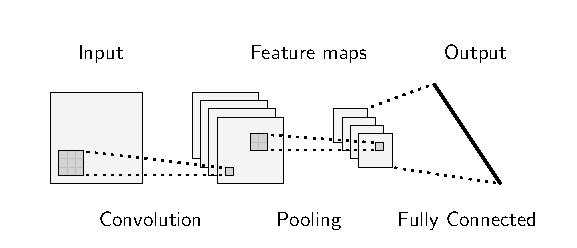
\includegraphics[scale=1]{figures/cnn.eps}
\caption{Typical convolutional neural network. }
\label{fig:typical_cnn}
\end{figure}

A pooling function replaces the output of the network at a certain location with a summary statistic of the nearby outputs. For example, the max pooling \cite{Zhou1988} operation reports the maximum output within a rectangular neighborhood. In this way, pooling helps to make the representation approximately invariant to small translations of the input. Invariance to translation means that when a input is translated by a small amount, the values of most of the pooled outputs do not change.

% In the context of machine learning, the learning algorithm will learn the appropriate values of the filter. 

% Convolutional neural networks (CNNs) \cite{LeCun1989} have been applied to sequences for decades. They were used prominently for speech recognition in the 80s and 90s.


\subsection{Recurrent Neural Networks}

In deep learning, a recurrent neural network (RNN) \cite{Rumelhart1988} is a class of artificial neural networks where connections between nodes form a directed graph along a temporal sequence. Unlike feedforward neural networks, RNNs contain cycles and use an internal state memory $\mathbf h$ to process sequences of inputs \cite{Elman1990}. A universal recurrent neural network is described by the propagation equations,
\begin{align}
\mathbf h_t &= \text{Activation}(\mathbf U \,\mathbf x_t + \mathbf W \, \mathbf h_{t-1} + \mathbf b) \\
\mathbf o_t &= \mathbf V \, \mathbf h_t + \mathbf c 
\end{align} 
where the parameters are the bias vectors $\mathbf b$ and $\mathbf c$ along with the weight matrices $\mathbf U$, $\mathbf V$ and $\mathbf W$, respectively, for input-to-hidden, hidden-to-output and hidden-to-hidden connections. The recurrent network maps an input sequence $\mathbf x_{1:T}$ of length $T$ to an output sequence $\mathbf o_{1:T}$ of the same length. The computational graph and its unfolded version is shown in Fig. \ref{fig:rnn}.
\begin{figure}[htbp]
\centering
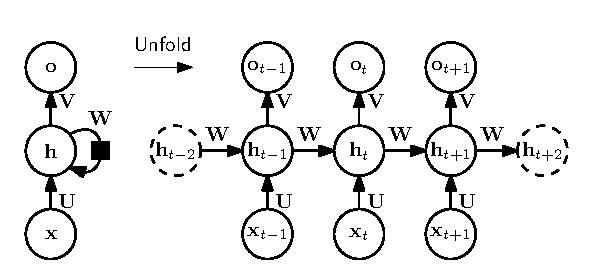
\includegraphics[scale=1]{figures/rnn.eps}
\caption{The computational graph on an recurrent neural network and its unfolded version.}
\label{fig:rnn}
\end{figure}    

Computing the gradients involves performing a forward propagation pass through the unrolled graph followed by a backward propagation pass. The runtime is $O(T)$ and cannot be reduced by parallelization because the forward propagation graph is inherently sequential, i.e., each time step may be computed only after the previous one. Therefore, back-propagation for recurrent model is called back-propagation through time (BPTT). Recurrent models construct very deep computational graphs by repeatedly applying the same operation at each time step of a long temporal sequence. This gives rise to the vanishing and exploding gradient problem and makes it notoriously difficult to train RNNs. To prevent these difficulties more elaborate recurrent architectures were developed, such as the LSTM \cite{Hochreiter1997} and the GRU \cite{Cho2014}. These families of architectures have gained tremendous popularity due to prominent applications to language modeling and machine translation. 

\paragraph{LSTM}
The long short-term memory (LSTM) \cite{Hochreiter1997} is an recurrent neural network (RNN) architecture used in the field of deep learning. It comprises leaky units to allow the network to accumulate information over a long duration. However, once that information has been used it might be useful for the network to forget the old state. Instead of manually deciding when to clear the state, the neural network learns to decide when to do it. The time scale of integration can be changed dynamically by making the weights gated, i.e., controllable by another hidden unit.

\paragraph{GRU}
The gated recurrent unit (GRU) \cite{Cho2014} is a gating mechanism in recurrent neural networks. The GRU is similar to an LSTM with forget gate but has fewer parameters than an LSTM, as it lacks an output gate. GRUs have been shown to exhibit even better performance on certain smaller datasets \cite{Chung2014}. However, the LSTM is strictly stronger than the GRU as it can easily perform unbounded counting, while the GRU cannot \cite{Weiss2018}.

% The intuitive appeal of recurrent modeling is that the hidden state can act as a representations of everything that has been seen so far in the sequence.

% Recurrent networks are dedicated sequence models that maintain a vector of hidden activations that are propagated throgh time \cite{Elman1990,Werbos1990,Graves2012}.






\subsection{Temporal Convolutional Networks}

A temporal convolutional network (TCN) \cite{Bai2018} represents a special architecture of convolutional neural network and is informed by recent convolutional architectures for sequential data. It is designed from first principles and combines simplicity, autoregressive prediction, and very long memory. In comparison to WaveNet \cite{Oord2016}, the TCN does not employ skip connections across layers (no conditioning, context stacking, or gated activations).

The TCN is based upon two principles: 1) the convolutions are casual, i.e, no information leakage from future to past; 2) the architecture can take a sequence of any length and map it to an output sequence of the same length just as with an RNN. To achieve the first point, the TCN uses a 1D fully-convolutional network architecture \cite{Long2015}, where each hidden layer is the same length as the input layer. To accomplish the second point, the TCN uses causal convolutions, i.e., convolutions where an output at time $t$ is convolved only with elements from time $t$ and earlier in the previous layer.

Simple causal convolutions have the disadvantage to only look back at history with size linear in the depth of the network. To circumvent this fact, the architecture employs dilated convolutions that enable an exponentially large receptive field. More formally, for a input sequence $\mathbf x \in \mathbb R^T$ and a filter $f:\{ 0, \dots, k-1\} \rightarrow \mathbb R$, the dilated convolution operation $F$ on element $s$ of the sequence is defined as
\begin{align}
F(s) = (\mathbf x *_d f)(s) = \sum_{i=0}^{k-1} f(i) \, \mathbf x_{s-d\cdot i}
\end{align}
where $d = 2^\nu$ is the dilation factor, with $\nu$ the level of the network, and $k$ is the filter size. The term $s-d\cdot i$ accounts for the direction of the past. Dilation is equivalent to introducing a fixed  step between every two adjacent filter taps, as it can be seen in Fig. \ref{fig:dilated_convolutions}. Using larger dilation enables an output at the top level to represent a wider range of inputs, thus effectively expanding the receptive field of a CNN. There are two ways to increase the receptive field of a TCN: choosing lager filter sizes $k$ and increasing the dilation factor $d$, since the effective history of one layer is $(k-1) \, d$. 

\begin{figure}[htbp]
\centering
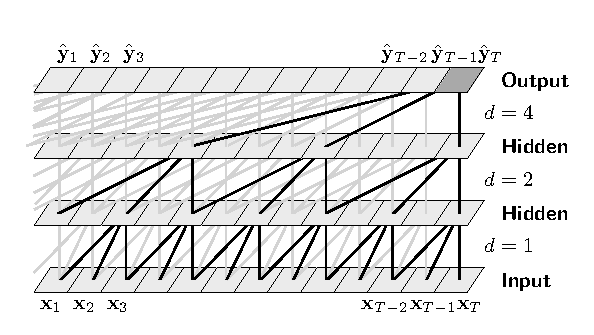
\includegraphics[scale=1]{figures/dilated_conv.eps}
\caption{A dilated casual convolution with dilation factors $d = 1,2,4$ and filter size $k=3$.}
\label{fig:dilated_convolutions} 
\end{figure}

Another architectural element of a TCN are residual connections. In place of a convolutional layer, TCNs employ a generic residual module. Each residual block contains a branch leading out to a series of transformations $\mathcal F$, whose outputs are added to the input $\mathbf x$ of the block 
\begin{align}
o = \text{Activation} \big(\mathbf x + \mathcal F(\mathbf x)\big)
\end{align}
This effectively allows layers to learn modifications to the identity mapping rather than the entire transformation, which has been shown to benefit deep neural networks \cite{He2016}. Especially for very deep networks stabilization becomes important, for example, in the case where the prediction depends on a large history size ($> 2^{12}$) with a high-dimensional input sequence. 

A residual block has two layers of dilated causal convolutions and rectified linear units (ReLU) as non-linearity, shown in Fig. \ref{fig:residual_block}. For normalization, weight normalization \cite{Salimans2016} is applied to the convolutional filters. In addition, a spatial dropout \cite{Srivastava2014} is added after each dilated convolution for regularization, i.e., at each training step, a whole channel is zeroed out.
\begin{figure}[htbp]
\centering
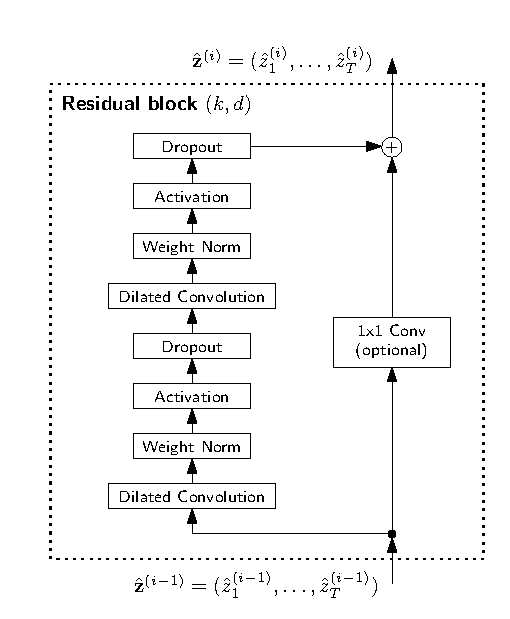
\includegraphics[scale=1]{figures/residual_block.eps}
\caption{TCN residual block.}
\label{fig:residual_block} 
\end{figure}


\begin{itemize}
\item the convolutions are casual, that means no information leakage from future to past (compare to bidirectional RNN).
\item long effective history sizes, i.e., the ability for networks to look very far into the past to make a prediction (receptive field?), by using a combination of very deep networks (augmented with residual layers) and dilated convolutions 
\item this allows layers to learn modifications to the identity mapping rather than the entire transformation, which has been shown to benefit deep neural networks (where?)
\item within a residual block there exist two layers of dilated causal convolution and a rectified linear unit (ReLU) \cite{Nair2010} as a non-linearity
\item for normalization a weight normalization \cite{Salimans2016} is applied to the convolutional filters 
\item additionally spatial dropout \cite{Srivastava2014} is added after each dilated convolution for regularization (at each training step, a whole channel is zeroed out)
\item The TCN architecture appears not inly more accurate than canonical recurrent networks such as LSTMs and GRUs, but also simpler and clearer.
\end{itemize}






\subsection{General-Purpose Computing on GPUs} 

In 2004, it was shown by K. S. Oh and K. Jung that standard neural networks can be greatly accelerated on GPUs. Their implementation was 20 times faster than an equivalent implementation on CPU \cite{Oh2004}. In 2005, another paper also emphasized the value of GPGPU for machine learning \cite{Steinkraus2005}.

While GPUs operate at lower frequencies, they typically have many times the number of cores. Thus, GPUs can process far more pictures and graphical data per second than a traditional CPU. Migrating data into graphical form and then using the GPU to scan and analyze it can create a large speedup.


\newpage


% Old: Beat Tracking System
\section{Method}

From an overall perspective, the proposed automatic beat tracking system comprises three major stages, as shown in Fig. \ref{fig:system}. In the first stage, the original audio is preprocessed. Data preprocessing refers to all transformations on the raw data before it is feed to the machine learning algorithm. It includes different methods such as normalization, transformation and feature extraction. 

\begin{figure}[htbp]
\centering
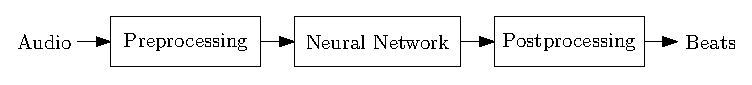
\includegraphics[scale=1.0]{figures/beat_tracking_system.eps}
\caption{Beat tracking system signal flow}
\label{fig:system}
\end{figure}  


\subsection{Dataset}
For training and evaluation we use the available datasets listed in Table \ref{tab:datasets}.
\begin{table}[htbp]
\caption{Datasets used for training.}
\label{tab:datasets}
\centering
\begin{tabular}{lrr}
\hline
\hline
\textbf{Dataset} & \textbf{files} & \textbf{length} \\
\hline
Ballroom \cite{Gouyon2006b, Krebs2013} & $685$ & $5\,\text{h} \;57\,\text{m}$\\
GTZAN \cite{Tzanetakis2002b, marchand2015swing} & $1000$ & $8\,\text{h}\;20\,\text{m}$\\
Hainsworth \cite{Hainsworth2004} & $222$ & $3\,\text{h}\;19\,\text{m}$\\
SMC \cite{Holzapfel2012} & $217$ & $2\,\text{h}\;25\,\text{m}$\\    
\hline
Total & $ $ & $ \,\text{h}\; \,\text{m}$\\  
\hline
\hline
\end{tabular}
\end{table}  

\paragraph{Ballroom} 
The Ballroom dataset \cite{Gouyon2006b, Krebs2013} contains 685 audio files\footnote{After removing the 13 duplicates which are pointed out by Bob Sturm \cite{Sturm2014}.} of ballroom dancing music. As genres the files cover Cha Cha, Jive, Quickstep, Rumba, Samba, Tango, Viennese Waltz, and Slow Waltz. Each file is $30\,\text{s}$ long, mono and sampled at $44.1\,\text{kHz}$ with $16\text{-bit}$ resolution.

\paragraph{GTZAN} 
The GTZAN \cite{Tzanetakis2002b} dataset was originally proposed for music genre classification problem and later extended with beat annotations \cite{marchand2015swing}. The dataset comprises 1000 excerpts of 10 different genres. The genres are blues, classical, country, disco, hip-hop, jazz, metal, pop, reggae and rock. Each file is $30\,\text{s}$ long, mono and sampled at $22050\,\text{Hz}$ with $16\text{-bit}$ resolution. The audio content of the GTZAN dataset is representative of the real commercial music of various music genre. The dataset has a good balancing between tracks with swing (Blues and Jazz music) and without swing.

\paragraph{Hainsworth} 
The Hainsworth dataset \cite{Hainsworth2004} contains 222 musical audio files, with the following genre breakdown: Rock/Pop (68), Dance (40), Jazz (40); Classical (30), Folk (22), and Choral (22). Each file is between $30$ and $60\,\text{s}$ in length, mono and sampled at $44.1\,\text{kHz}$ with $16\text{-bit}$ resolution.

\paragraph{SMC}
The SMC dataset \cite{Holzapfel2012} contains 217 musical audio files. Each file is $40 \,\text{s}$ in length, mono and sampled at $44.1\,\text{kHz}$ with $16\text{-bit}$ resolution.


\subsection{Data Preprocessing}

The training dataset contains raw pulse code modulated (PCM) audio signals stored as WAV files. For the sake of consistency and also to reduce computational complexity, every audio signal is resampled at a sampling rate $f_s = 44.1 \,\text{kHz}$ with $16\text{-bit}$ resolution and converted to a monaural signal by averaging both stereo channels. 

In complex polyphonic mixtures of music, simultaneously occurring events of high intensities lead to masking effects that prevent any observation of an energy increase of a low intensity onset \cite{Grosche2010}. To circumvent these masking effects, the signal is analyzed in a band-wise fashion to extract transients occurring in certain frequency regions of the signal. Therefore, a filtered frequency spectrum is chosen to serve as the input for the neural network.


\paragraph{Input}

The discrete audio signal $x(n)$ is segmented into overlapping frames of $N = 2048$ samples, which corresponds to a length of $46.4 \,\text{ms}$. The frames are sampled every $10 \,\text{ms}$, resulting in a frame rate $f_r = 100 \,\text{fps}$. A standard Hamming window $w(n)$ of the same length is applied to the frames before the short-time Fourier transform (STFT) is used to compute the complex spectrogram 
\begin{align}
X(t,\omega) = \sum_{n = 1}^{N} w(n) \, x(n + t\,h) \, e^{-2 \pi j \omega /N}
\end{align} 
where $t$ refers to as the frame index, $\omega$ the frequency bin index, and the hop size $h=441$, i.e., the time shift in samples between adjacent frames. The complex spectrogram $X(t,\omega)$ is converted to the power spectrogram $|X(t,\omega)|^2$ by omitting the phase portion of the spectrogram. The power spectrogram is filtered with a bank of overlapping triangular filters $F(t,\omega)$ with 12 bands per octave covering a frequency range of $30$ to $17,000 \, \text{Hz}$. To better match the human perception of loudness, a logarithmic representation is chosen, 
\begin{align}
S(t,\omega) = \log \left( |X(t,\omega)|^2 \cdot F(t,\omega)^T + 1 \right)
\end{align} 
At every time instant $t$ the input  $\mathbf x_t \in \mathbb R^n$ to the neural network corresponds to the frequency column of the filtered log power spectrogram $S(t,\omega)$
\begin{align}
\mathbf x_t = S(t,\omega), \quad \forall\, t= 1,\dots,T
\end{align} 
and has dimensionality $n=88$.
% ``Is it important to use several features?'' [Durand2015]
% Two different types of input features: Onset events and harmonic changes
% Assumtion: Most harmonic changes occur inside a piece of music are located at metric bars \cite{Khadkevich2012}
% https://musicinformationretrieval.wordpress.com/2017/04/25/audio-beat-tracking-human-annotation-strategies/


\paragraph{Labels}
The beat tracking task requires annotations in the form of time instants of beats from a musical excerpt. To this end, the beat tracking problem is considered as a binary classification problem, where annotated beat instants are first quantized to the temporal resolution of the input representation, and then represented as training targets $y_{1:T}$. Following the strategy of onset detection \cite{Schluter2014} the temporal activation region around the annotations is widen by means of including two adjacent temporal frames on either side of each quantized beat location and weight them with a value of $0.5$ during training. 


% \paragraph{Training Set} 
% After preprocessing the audio data, we obtain the training set $ O = \left\{ \mathbf x^{(\alpha)}, \, y^{(\alpha)} \right \}_{\alpha = 1}^p$, with $p$ samples in total. 


\paragraph{Chroma Representation}

\begin{itemize}
\item Chords are more likely to change in beat times than on other positions. Chords are more likely to change at the beginnings of measures than at other positions of the beat.
\item A chromagram comprises a time-series of chroma vectors, which represent harmonic content at a specific time in the audio.
\item Chromagrams are concise descriptors of harmony because they encode tone quality and neglect tone height.
\item CRP (chroma DCT-reduced log-pitch) features have significant amount of robustness to changes in timbre an instrumentation \cite{Mueller2010}.
\item Employ data-driven approach to extract chromagrams that specifically encode content relevant to harmony.
\item Chroma features are noisy in their basic formulation be- cause they are affected by various interferences: musical instruments produce overtones in addition to the fundamental frequency; percussive instruments pollute the spectrogram with broadband frequency activations (e.g. snare drums) and/or pitch-like sounds (tom-toms, bass drums); different combinations of instruments (and different, possibly genre-dependent mixing techniques) create different timbres and thus increase variance \cite{Korzeniowski2016}.
\end{itemize}


\subsection{Feature Learning}
From an overall perspective, the neural network architecture consist of two main blocks, as it is shown in Fig. \ref{fig:neural_net}. While the filtered log power spectrum could be passed directly to the TCN, the network first seeks to learn some compact intermediate representation, by implementing a preceding convolutional block. To capture the sequential structure, a TCN finally transforms the intermediate representation $\mathbf z_{1:T}$ directly into a sequence of beat activations $a_{1:T}$.
\begin{figure}[htbp]
\centering
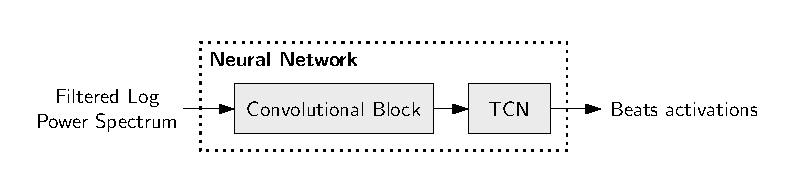
\includegraphics[scale=1.0]{figures/neural_net.eps}
\caption{Neural network}
\label{fig:neural_net}
\end{figure}    

The convolutional block is a set of convolution and max pooling layers and reduce the dimensionality both in time and frequency. The convolutional layers contain $16$ filters each, with kernel sizes of $3\times3$ for the first two, and $1\times8$ for the last layer, as it is shown in Fig \ref{fig:conv_block}. The intermediate max pooling layers apply pooling only in the frequency direction over $3$ frequency bins. A dropout \cite{Tompson2015} rate of $0.1$ is used with the exponential linear (ELU) \cite{Clevert2015} as activation function.
\begin{figure}[htbp]
\centering
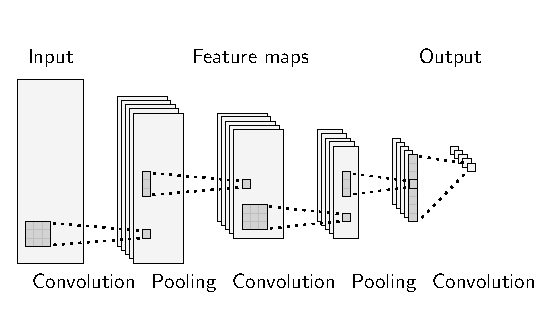
\includegraphics[scale=1.0]{figures/conv_block.eps}
\caption{Convolutional Block}
\label{fig:conv_block}
\end{figure}    

The output of the convolutional block $\mathbf z_t$ is a 16-dimensional feature vector and serves as the input to the TCN. The TCN is constructed as stacked residual blocks, as shown in Fig. \ref{fig:residual_block}, and contains $11$ layers with 16 filters of size $5$ and geometrically spaced di\-lations ranging from $2^0$ up to $2^{10}$ time frames. Thus, the resulting receptive field is approximately $81.5\,\text{s}$. A spatial dropout with rate $0.1$ and the ELU activation function is used. The output layer of the TCN has two units, representing the two classes ``beat'' and ``no beat''. Thus, the network can be trained as a binary classifier with the cross entropy error function. The outputs use the log softmax activation function, 
\begin{align}
\log \text{softmax}(x_i) = \log\left(\frac{\exp{(x_i)}}{\sum_j \exp(x_j)}\right)
\end{align} 
which is added to the last layer of the neural network. Therefore, the output $\hat{\mathbf y}_t = (\hat{y}_{1_t}, \hat{y}_{2_t})^T$ represent the log-probabilities for the two classes at time $t$. Finally, the beat activation $a_t$ can be calculated by
\begin{align}
a_t = \exp \left({\hat{y}_{1_t}} \right), \quad \forall \, t= 1,\dots,T
\end{align}  
which represent the probability of a beat at each frame.

The final model is trained with the ADAM optimizer \cite{Kingma2014} with a batch size $M = 20$ and a learn rate of $\mu = 1 \,e^{-3}$. The whole system has only $30818$ trainable parameters. 

% Seuqence-to-sequence prediction: the entire input sequence can be used to predict each output (not feasible in real time processing)
% Binary classification problem: beat (class 1); no beat (class 0)


\subsection{Temporal Decoding}
\label{sec:temporal_decoding}

The metrical structure of music builds upon a hierarchy of approximate regular pulses, as elaborated in Section \ref{sec:perception}. To exploit this sequential structure, a probabilistic dynamic model is used to result in a more robust estimation of the beat instants and to correctly operate under rhythmic fluctuations, such as ritardando and accelarando or metric modulations.

As a post-processing stage following the feature learning, a dynamic Bayesian network (DBN) is employed which jointly infers tempo and the phase of the beat. Dynamic Bayesian networks are popular frameworks for meter tracking in music because they are able to incorporate prior knowledge about the dynamics of rhythmic parameters. 
In this DBN, which is a hidden Markov model (HMM) precisely, a sequence of hidden variables that represent the meter of an audio piece is inferred from a sequence of observed variables. The probabilistic state space consist of two hidden variables, the position within a bar and the tempo. 

The probabilistic model is based upon the bar pointer model of Whiteley et al. \cite{Whiteley2006} which enables joint inference of rhythmic parameters from a piece of music. Mutual dependencies between these parameters are exploited, which increases the computational complexity of the models. A bar pointer is defined as being a hypothetical hidden object located in state space consisting of the period of a latent rhythmical pattern. The velocity of the bar pointer is defined to be proportional to tempo. The advantage of this approach is that the bar pointer continues to move whether or not a beat activation is observed. This explicitly models the concept that meter is a latent process and provides robustness against rest in the music which might otherwise be wrongly interpreted as local variations in tempo. In order to make inference computationally tractable, the state-space is usually divided into discrete cells \cite{Krebs2015}. 

Given a sequence of observed data $a_{1:T}$, we wish to identify the most probable hidden state trajectory $\mathbf s_{1:T}$. At each time frame $t$, the bar pointer of the hidden state space is referred to as $\mathbf s_t = [\phi_t, \nu_t]$, with $\phi_t \in \{1, 2, \dots, K\}$ denoting the position within a bar, and $\nu_t \in \{ K_{\text{min}}, K_{\text{min}}+1, \dots, K_{\text{max}}\}$ referring to as the tempo. The number of discrete bar positions $K$ is dependent on the tempo by using exactly one bar position state per audio frame and thus per observation feature value. The number of observations per bar (four beats) at a tempo $\Theta$ in beats per minute (BPM) is
\begin{align}
K(\Theta) = \left\lfloor \frac{4 \times 60}{\Theta \, \Delta} \right\rfloor 
\label{eq:number_of_obstervations_per_bar}
\end{align} 
where $\Delta$ is referred to as the audio frame length. With Equation. \ref{eq:number_of_obstervations_per_bar}, one can compute the number of bar positions of the tempo limits $K_\text{min} = K(\Theta_\text{max})$ and $K_\text{max} =K(\Theta_\text{min})$. Using a tempo range of  $\Theta = [55, 215]$ the position within a bar has at most $82$ tempo states.

With this state space discretization, the most likely hidden state sequence $\mathbf s_{1:T}^* = \mathbf s_1^*, \dots, \mathbf s_T^*$ given a sequence of observations $a_{1:T} = a_1, \dots, a_T$ is computed by
\begin{align}
\mathbf s_{1:T}^* = \arg \max_{\mathbf s_{1:T}} P(\mathbf s_{1:T}\,|\, a_{1:T})
\label{eq:most_likely_states}
\end{align} 
with 
\begin{align}
 P(\mathbf s_{1:T}\,|\, a_{1:T}) \propto P(\mathbf s_1) \prod_{t=2}^T P(\mathbf s_t\,|\,\mathbf s_{t-1})\, P( a_t\,|\,\mathbf s_{t})
\end{align} 
where $P(\mathbf s_1)$ is the initial state distribution, $P(\mathbf s_t\,|\,\mathbf s_{t-1})$ is the transition model, and $P(\mathbf a_t\,|\,\mathbf s_{t})$ is the observation model. The most likely hidden state sequence can be solved using the well-known Viterbi algorithm \cite{Viterbi1967}. Finally, the set of beat instant $\mathcal B$ can be extracted from the sequence of bar positions as
\begin{align}
\mathcal B = \{ t: \phi_t^*=1\}
\end{align} 
In order to infer the hidden variables from an audio signal, the three entities are specified. The transition model describes the transitions between the hidden variables. The observation model takes the beat activations from the neural network
and initial distribution encodes prior knowledge about the hidden variables.

\paragraph{Initial Distribution} 
Any prior knowledge about tempo distributions can be incorporated into the model. For example, if the music to be tracked from one genre, a specific tempo distribution can be used. To make it genre independent, a uniform distribution is used in this theses. 


\paragraph{Transition Model} The transition model $P(\mathbf s_t\,|\,\mathbf s_{t-1})$ can be further decomposed into a distribution for each of the two hidden variables $\phi_t$ and $\nu_t$, this is
\begin{align}
P(\mathbf s_t\,|\,\mathbf s_{t-1}) = P(\mathbf \phi_t\,|\,\mathbf \phi_{t-1}, \nu_{t-1}) \, P(\nu_t \, |\, \nu_{t-1}) 
\end{align} 
where the first factor is
\begin{align}
P(\mathbf \phi_t\,|\,\mathbf \phi_{t-1}, \nu_{t-1}) = \mathbf 1_A
\end{align} 
with the indicator function $\mathbf 1_A$ that equals one if $\phi_t = (\phi_{t-1}+\nu_{t-1}-1)\mod M+1$. The modulo operator makes the bar position cyclic. If $\phi_t \in \mathcal B$, the second factor is defined by
\begin{align}
P(\nu_t \, |\, \nu_{t-1}) = \exp \left( -\lambda \left| \frac{\nu_{t}}{\nu_{t-1}} -1 \right| \right)
\end{align} 
otherwise it is
\begin{align}
P(\nu_t \, |\, \nu_{t-1}) = \begin{cases}
    1, &\nu_t = \nu_{t-1}\\
    0, &\text{else.} 
\end{cases}
\end{align} 
The parameter $\lambda \in \mathbb Z_{\geq0}$ determines the steepness of the distribution and models the probability for a tempo change. A value of $\lambda = 0$ means that transitions to all tempi are equally probable. In practice, for music with roughly constant tempo, we set $\lambda \in [1, 300]$. The probability of tempo change is heuristically set to $p_\omega = 0.002$. Higher-level or domain specific knowledge could be used to set this parameter. For example in rock or pop music, the beat is usually quite steady, so a small value for $p_\omega$ would be quite appropriate, while for classical music, particularly styles including many tempo changes, a higher value would be more optimal.


\paragraph{Observation Model}
The beat activation function produced by the neural network is limited to the range $[0, 1]$ and shows high values at beat positions and low values at non-beat positions. Thus, the activation function is used directly as state-conditional observation distributions \cite{Degara2012}. The observation likelihood is defined as 
\begin{align}
P(a_t\,|\,\phi_t) = \begin{cases}
    a_t, &1 \leq \phi_t\leq \frac{\lambda}{\Lambda}\\
    \frac{1-a_t}{\lambda-1}, &\text{else}.    
\end{cases}
\end{align} 





% \subsection{Time-Frequency Reassignment}
% \begin{itemize}
% \item audio signals have a distribution of energy that varies in time and frequency
% \item a spectrogram is constrained by an unfortunate tradeoff between resolution in time and frequency
% \item time-frequency reassignment: mapping the data to time-frequency coordinates that are nearer to the true region of support of the analyzed signal
% \item time-frequency reassignment has been used in a variety of applications for obtaining improved time and frequency estimates for time-varying spectral data [cite... 16-18]
% \end{itemize}



\newpage
\section{Evaluation}

Robust evaluation is inevitable, not only to determine the individual successes and failures of the algorithm, but also to measure its relative performance among different algorithms. With the development of the Music Information Retrieval Evaluation eXchange (MIREX) \cite{Downie2008}, evaluation has become a fundamental aspect of research in music information retrieval. MIREX represents a community-based formal evaluation framework for the evaluation of algorithms and techniques related to music information retrieval.  

In this section, existing objective evaluation methods are reviewed, and applied to the proposed beat tracking system. The result is compared against the current state-of-the-art algorithm in beat tracking, which is freely available within the Madmom Python library \cite{Boeck2016}.


% Discontinuity in the pulse see Gouyon2005 page 3

%  annotations tapped at different metrical levels in beat tracking

% objective methods for beat tracking evaluation compare the output beat times from a beat tracking algorithm against one or more sequences of ground truth annotated beat times. \cite{Davies2009b}
% We must question the importance of strict continuity when evaluating a beat tracking system. A single misplaced beat, in the context of a sequence of otherwise accurate beats, is a far less disturbing error than the accuracy calculated with the continuity requirement would suggest. 


\subsection{Evaluation Methods}

The choice of evaluation method can have a significant impact on the relative performance of different beat tracking algorithms. An evaluation method should adequately contend with the inherent uncertainty or ambiguity while providing a measurement of performance which is both meaningful and easy to interpret \cite{Davies2009b}. 

Each evaluation method takes a set of annotated beat times $\mathcal A = \{a_1, \dots, a_A\}$ and a corresponding set of predicted beat times $\mathcal B = \{b_1, \dots, b_B\}$, where $A$ refers to the number of annotations, and $B$ to the number of annotations, respectively.


\paragraph{F-measure} 
In statistical analysis of binary classification, the F-measure, also called the $F_1$ score, is a generic measure to test accuracy. It considers both the precision $p$ and the recall $r$ of the test to compute the score. The precision $p$ is the number of true positives $tp$ divided by the number of all positive results returned by the classifier, i.e, the number of true positives $tp$ plus the number of false positives $fp$
\begin{align}
p = \frac{tp}{tp + fp}
\end{align} 
The recall $r$ is referred to as the number of true positives $tp$ divided by the number of all relevant samples, i.e, all samples that should have been identified as positive
\begin{align}
r = \frac{tp}{tp + fn}
\end{align} 
The F-measure is the harmonic mean of the precision and recall
\begin{align}
F_1=  \frac{2\,p\, r}{p +r} = \dfrac{2\, tp}{2\, tp + fp + fn}
\end{align} 
where an F-measure reaches its best value at 1 (perfect precision and recall) and worst at 0. In beat tracking, a result is regarded as true positive if a detected beat is in $\pm 70\,\text{ms}$ rage of an annotated beat. One can understand, the number of false positives as extra detections of the system, while the number of false negatives correspond to the missed detections.



\paragraph{Continuity measures} 
In contrast to the F-measure, where the accuracy is determined from the overall beat tracking success, Hainsworth \cite{Hainsworth2004b} and Klapuri et al. \cite{Klapuri2006} developed evaluation methods, which measure the success of regions of continuously correctly tracked beats. Continuity is enforced by the implementation of tolerance windows of $\theta  = \pm 17.5\, \%$ of the current inter-annotation-interval around each annotation. The closest detected beat to each annotation can only be correct if it falls within this tolerance window and the previous detected beat is also within the tolerance window of the previous annotation. This condition addresses beat phase, but also requires consistency between inter-annotation-intervals. 

Comparing each detected beat $b_i$ to each annotation $a_j$, there is a number of correct beats in each continuously correct segment $Y_m$, where there are $M$ continuous segments. The ratio of the longest continuously correct segment to the length of the annotations $J$ defines the correct metrical level with continuity required
\begin{align}
\label{eq:CMLc}
\text{CML}_\text{c} = \frac{\max(Y_m)}{J}
\end{align} 

CMLc only reflects information about the longest segment of correct beat tracking. Therefore, it does not include the contribution of any other beats which may also be correct. For example, if a single wrong detected beat occurs and this beat error happens to be in the middle of the excerpt, this would lead to $\text{CML}_\text{c} = 0.5$. To include the effect of beats in other segments $Y_m$, a less strict measure is the total number of correct beats at the correct metrical level
\begin{align}
\label{eq:CMLt}
\text{CML}_\text{t} = \frac{\sum_{m=1}^MY_m}{J}
\end{align} 

To account for ambiguity in metrical levels, equations (\ref{eq:CMLc}) and (\ref{eq:CMLt}) are recalculated such that the annotation sequence a can be resampled to permit accurate tapping at double or half the correct metrical level and to allow for off-beat tapping. These conditions are referred to as allowed metrical level, which result in the two measures, allowed metrical levels continuity required ($\text{AML}_\text{c}$), and allowed metrical levels continuity not required ($\text{AML}_\text{t}$). 

\paragraph{Information Gain}
Davies et al. \cite{Davies2009b} developed an evaluation method without reliance on tolerance windows, by measuring the timing error between beats and annotations. The information gain $D$ is a measure of how much information the beats provide about the annotations. To this end, a error histogram with $K$ bins is formed from the resulting timing error sequence. The numerical score is then calculated as the Kullback-Leibler divergence with respect to a uniform histogram. The range for the information gain is $0\,\text{bits}$ to approximately $5.3\,\text{bits}$, where the upper limit is determined as $\log_2(K)$. An information gain of $0\,\text{bits}$ is obtained, when the beat error histogram is uniform, i.e. where the beat sequences are totally unrelated.



% \paragraph{P-score:} Define two sequences $T_a$ and $T_b$ as 

% $T_a(n) = \begin{cases}
% 	1, &\text{ if } n \in \mathcal A \\
% 	0 , & \text{ otherwise }
% \end{cases}, \qquad T_b(n) = \begin{cases}
% 	1, &\text{ if } n \in \mathcal B \\
% 	0 , & \text{ otherwise }
% \end{cases}$

% $\text{P-score} = \dfrac{\displaystyle \sum_{m=-w}^w  \sum_{n}\,  T_a(n)\,  T_b(n+m)}{\max(A,B)} \;, \qquad \text{where } w = 0.2 \, \text{median}(\Delta_a)$ 


\subsection{Results}
The performance of the proposed beat tracking system is determined using different evaluation methods, which are applied to the subsets of the training set. The achieved performance is compared against the state-of-the-art beat tracker from Böck et al. \cite{Boeck2014}. The overview of the performances of both beat tracking algorithms is shown in Tab. \ref{tab:performance}.
\begin{table}[htbp]
\caption{Overview of beat tracking performance}
\label{tab:performance}
\centering
\begin{tabular}{lcccccc}
\hline \hline
& F-Measure & CMLc & CMLt & AMLc & AMLt & D
\vspace{0.0em}\\\hline \vspace{-0.6em}
\csvreader[head to column names, filter equal={\dataset}{1}]{/Users/juliusrichter/Documents/Uni/Masterarbeit/beat_tracker/data/performance.csv}{}
{\\\name & \Fmeasure & \CMLc & \CMLt & \AMLc & \AMLt & \D}
\vspace{0.2em}\\\hline \vspace{-0.6em}
\csvreader[head to column names, filter equal={\dataset}{2}]{/Users/juliusrichter/Documents/Uni/Masterarbeit/beat_tracker/data/performance.csv}{}
{\\\name & \Fmeasure & \CMLc & \CMLt & \AMLc & \AMLt & \D}
\vspace{0.2em}\\\hline \vspace{-0.6em}
\csvreader[head to column names, filter equal={\dataset}{3}]{/Users/juliusrichter/Documents/Uni/Masterarbeit/beat_tracker/data/performance.csv}{}
{\\\name & \Fmeasure & \CMLc & \CMLt & \AMLc & \AMLt & \D}
\vspace{0.2em}\\\hline \vspace{-0.6em}
\csvreader[head to column names, filter equal={\dataset}{4}]{/Users/juliusrichter/Documents/Uni/Masterarbeit/beat_tracker/data/performance.csv}{}
{\\\name & \Fmeasure & \CMLc & \CMLt & \AMLc & \AMLt & \D}
\vspace{0.2em}\\\hline \hline
\end{tabular}
\end{table}




\subsection{Saliency Maps}

\begin{itemize}
\item Artificial neural networks often give good results, but it is difficult to understand what they learned, or on which basis they generate their output.
\item Compute saliency maps using guided back-propagation \cite{Springenberg2014}
\item How do the filters of the convolutional block look like?
\end{itemize}



\subsection{Network Training}

\begin{itemize}
\item Conclusion by Korzeniowski: To achieve better results, we could use DNN ensembles instead of a single DNN. We could ensure that the network sees data for which its predictions are wrong more often during training, or similarly, we could simulate a more balanced dataset by showing the net super-frames of rare chords more often \cite{Korzeniowski2016}
\end{itemize}



\subsection{Labeling}

\begin{itemize}
\item Enhance beat annotations the Sonic Visualiser \cite{SonicVisualiser} editor, that enables a user to mark beat positions in a digitalized audio signal while listening to the audio and watching its waveform.
\item The positions can be finely adjusted by playing back the audio with click tones at beat times.
\item The audio excerpt in time domain and its spectrogram can be visualized using tools like Sonic Visualiser. Beat locations can first be obtained by recording the tap locations the musical excerpt and then manually correcting these locations for exact onsets.  Annotators can also follow a semi-automatic process, for example in \cite{Peeters2010}, where beats and downbeats were first obtained through the Ircambeat software and then errors were manually corrected by human annotators.
\end{itemize}


\newpage 

\section{Conclusion}

\begin{itemize}
\item An efficient audio based beat tracking algorithm was presented, that is able to produce equivalent results to the current state-of-the-art. 
\item Causal model and less parameters in contrast to \cite{Boeck2014}.
\item Theoretically, a single network large enough should be able to model all different music styles simultaneously but unfortunately this optional solution is hardly achievable. The main reason for this is the difficulty to choose an absolutely balanced training set with an evenly distributed set of beats over all the different dimensions relevant for detecting beats. These include rhythmic patterns, harmonic aspects and many other features
\item Limitations in both the amount of training data and the variable quality of the annotations. Perform data augmentation. 
\item Dataset size: a rough rule of thumb is that a supervised deep learning algorithm will generally achieve acceptable performance with around 5000 labeled examples per category and will match or exceed human performance when trained with a dataset containing at least 10 million labeled examples \cite{Goodfellow2016}.
\item The most mentionable aspect is that the neural networks were trained solely on ballroom dance and other kinds of western pop music. The networks accuracy depends on the trainings set. Selective bias. 
\item Leave higher level analysis to the neural network
\item Take raw audio as input and learn Fourier transform with neural net.
\item System operates causally, thus an real-time implementation is possible.
\item Data augmentation (transformation or adding noise) $\Rightarrow$ prediction gets robust against transformation and noisy signals
\item Additionally, the tempo, metrical level of the beat and downbeat positions can also be annotated for related tasks like downbeat tracking/ meter tracking/ tempo tracking etc (multi-task learning) \cite{Boeck2019}.
\end{itemize}

\newpage

\section*{General notes}
\begin{itemize}
\item Goal of supervised learning: predict not yet observed input.
\item Motivation: ``\emph{It is probable that no universal beat tracking model exist which does not utilize a switching model to recognize style and context prior to application.}'' \cite{Collins2006}
\item Instead of calculating the STFT as for input features discover a good set of features by representation learning. (``\emph{Learned representations often result in much better performance than can be obtained with hand-designed representations.}'' \cite{Goodfellow2016})
\item Common association between sequence modeling and recurrent networks: ``\emph{Given a new sequence modeling task or dataset, which architecture should one use?}'' \cite{Bai2018}
\item Certain convolutional architectures can reach state-of-the-art accuracy in audio synthesis (e.g. Google WaveNet \cite{Oord2016})
\item Do TCNs outperform LSTM architectures in this particular sequence modeling task?
\item Contrast of the two statements:
\begin{itemize}
\item ``\emph{Feature extraction is an essential step towards effective and accurate beat/downbeat positions extraction.}'' \cite{Khadkevich2012}
\item ``\emph{The system shows state-of-the-art beat and downbeat tracking performance on a wide range of different musical genres and styles. It does so by avoiding hand-crafted features such as harmonic changes, or rhythmic patterns, but rather leans the relevant features directly from audio.}'' \cite{Boeck2016b}
\end{itemize} 
\item Hainsworth and MacLeaod state that beat tracking systems will have to be style specific in the future in order to improve the state-of-the-art \cite{Hainsworth2004}.
\item The no free lunch theorem for machine learning \cite{Wolpert1996} states that, averaged over all possible data-generating distributions, every classification algorithm has the same error rate when classifying previously unobserved points. This implies that we must design our machine learning algorithms to perform well on a specific task.
\item The method for obtaining ground truth annotations depends on whether the aim is to identify descriptive beat locations or to replicate a human tapping response. In the former case, an initial estimate of the beat locations can be obtained by recording tap times for a given musical excerpt and iteratively modifying and auditing the obtained beat positions while in the latter case, the ground truth can be completely defined by the tapping response \cite{Davies2009b}.
\item Due to uncertainties in the annotation process, for many types of input signals (especially multi-instrument excerpts) it may not possible to determine onset locations with greater precision than $50\,\text{ms}$. \cite{Leveau2004}
\item  The ideal outcome of the annotation is an unambiguous representation of the start points of musical events
\item Tried out Trellis Networks \cite{Bai2018b}, but not better than TCN. 
\end{itemize}


\newpage 
\bibliographystyle{unsrt}
\bibliography{references}

\end{document}